\documentclass{article}

\usepackage{graphicx, float, blindtext} % for dummy text
\usepackage{amsmath}
\graphicspath{ {./images/} }
\title{Chapter 10: Model comparison and Hierachical Modelling}
\author{Shubham Gupta}

\begin{document}
\maketitle
\section{Introduction}
\begin{itemize}
    \item When we have multiple models describing the same data, we need to assign credibilities to each model.
    \item Bayesian model comparison reallocates credibility across models given the data.  
    \item Model comparison $\implies$ bayesian estimatation of hierachical models where the top-level is the index of the models.
\end{itemize}
\section{Bayes Factor}
\subsection{General Formula}
\begin{itemize}
    \item Assume we have data $D$ with parameters $\theta$.
    \item Prior distribution is $p(\theta)$
    \item Parameter  $m$ to specify the index of the model.
    \item Hence, we will get
        \[
            likelihood = p_{m}(y|\theta_{m}, m)
        .\] 
        \[
            prior = p(\theta_{m}|m) 
        .\]                 

    \item Priors have different subscripts because they might have different distributions for each model.
    \item Assume each model is given a prior probability of $p(\theta)$. Then, for all possible models $\theta_{1}, \theta_{2}\ldots m$, we have:
        \[
            p(\theta_{1}, \theta_{2} \ldots | D) = \frac{P(D | \theta_{1}, \theta_{2} \ldots m) * p(\theta_{1}, \theta_{2} \ldots m)}{\sum_{m} \int d\theta_{m}p(D| \theta_{1}, \theta_{2} \ldots m) p(\theta_{1}, \theta_{2} \ldots m)} 
        .\] 
        \begin{figure}[H]
            \centering
            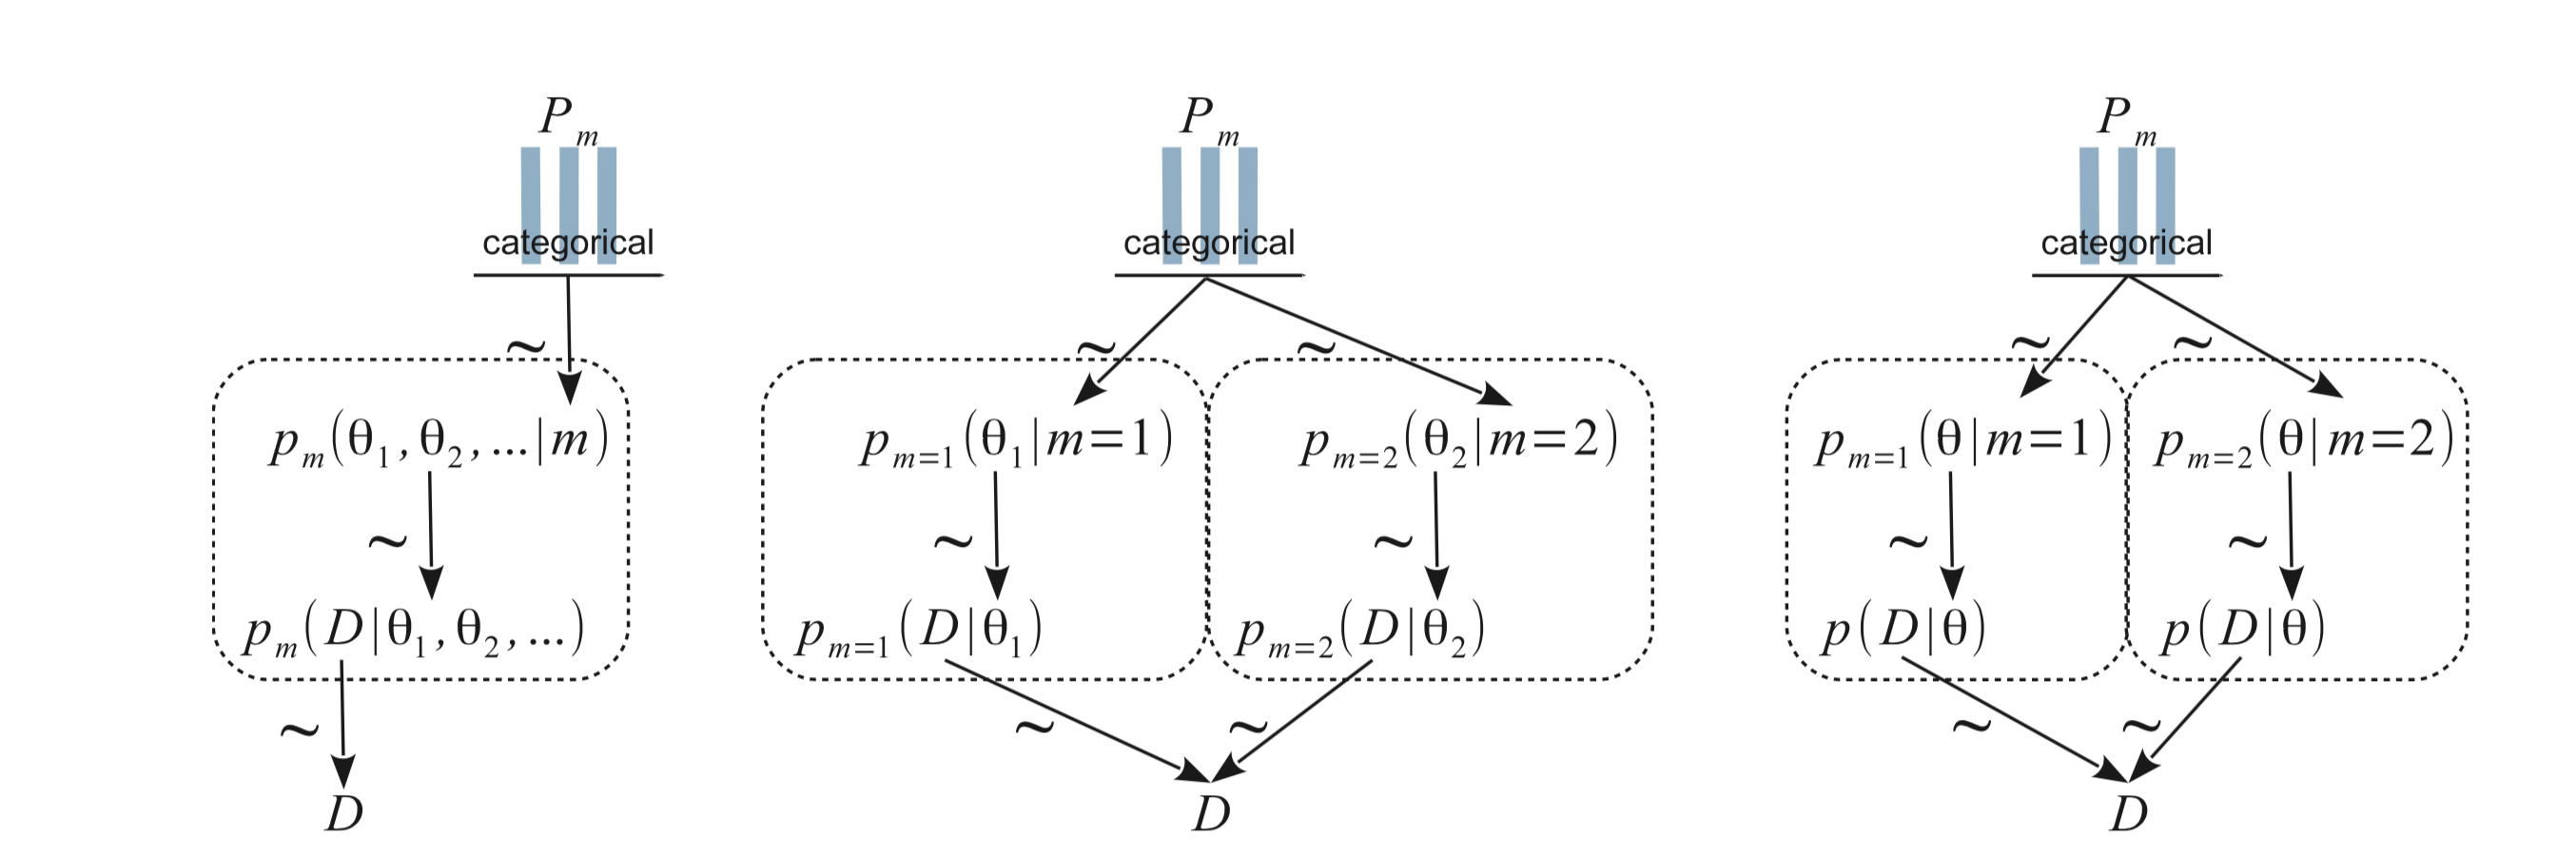
\includegraphics[width=0.8\textwidth]{model_index}
            \caption{Model comparisons as a hierachical model}
            \label{fig:model_index}
        \end{figure} 
    \item To get the relative probabilities of the models, we will divide their posterior outputs.
        \[
            \frac{p(m=1 | D)}{p(m=2 | D)} = \frac{p(D | m = 1) * p(m=1) / \sum_{m}P(D|m) * p(m)}{p(D | m = 2) * p(m=2) /\sum_{m}P(D|m) * p(m)}
        .\] 
    \item The above equation is called the Bayes Factor
    \item We can use the below table for reference on figuring out when to report a model is better than the alternative model.
        \begin{figure}[H]
            \centering
            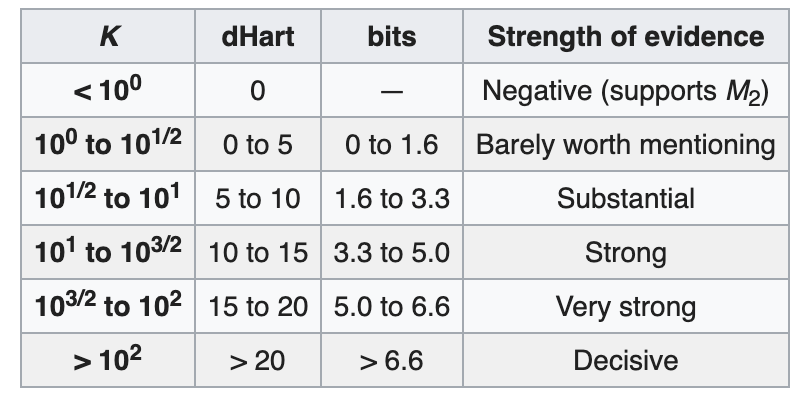
\includegraphics[width=0.8\textwidth]{bayes_factor}
            \caption{bayes factor}
            \label{fig:bayes_factor}
        \end{figure} 
\end{itemize}
\section{Head biased vs tail biased factories}
\begin{itemize}
    \item Two factories that produce head-biased and tail biased factories. Given we have seen some tosses, which factory did the coin come from?
    \item We have the following hierachy
        \begin{figure}[H]
            \centering
            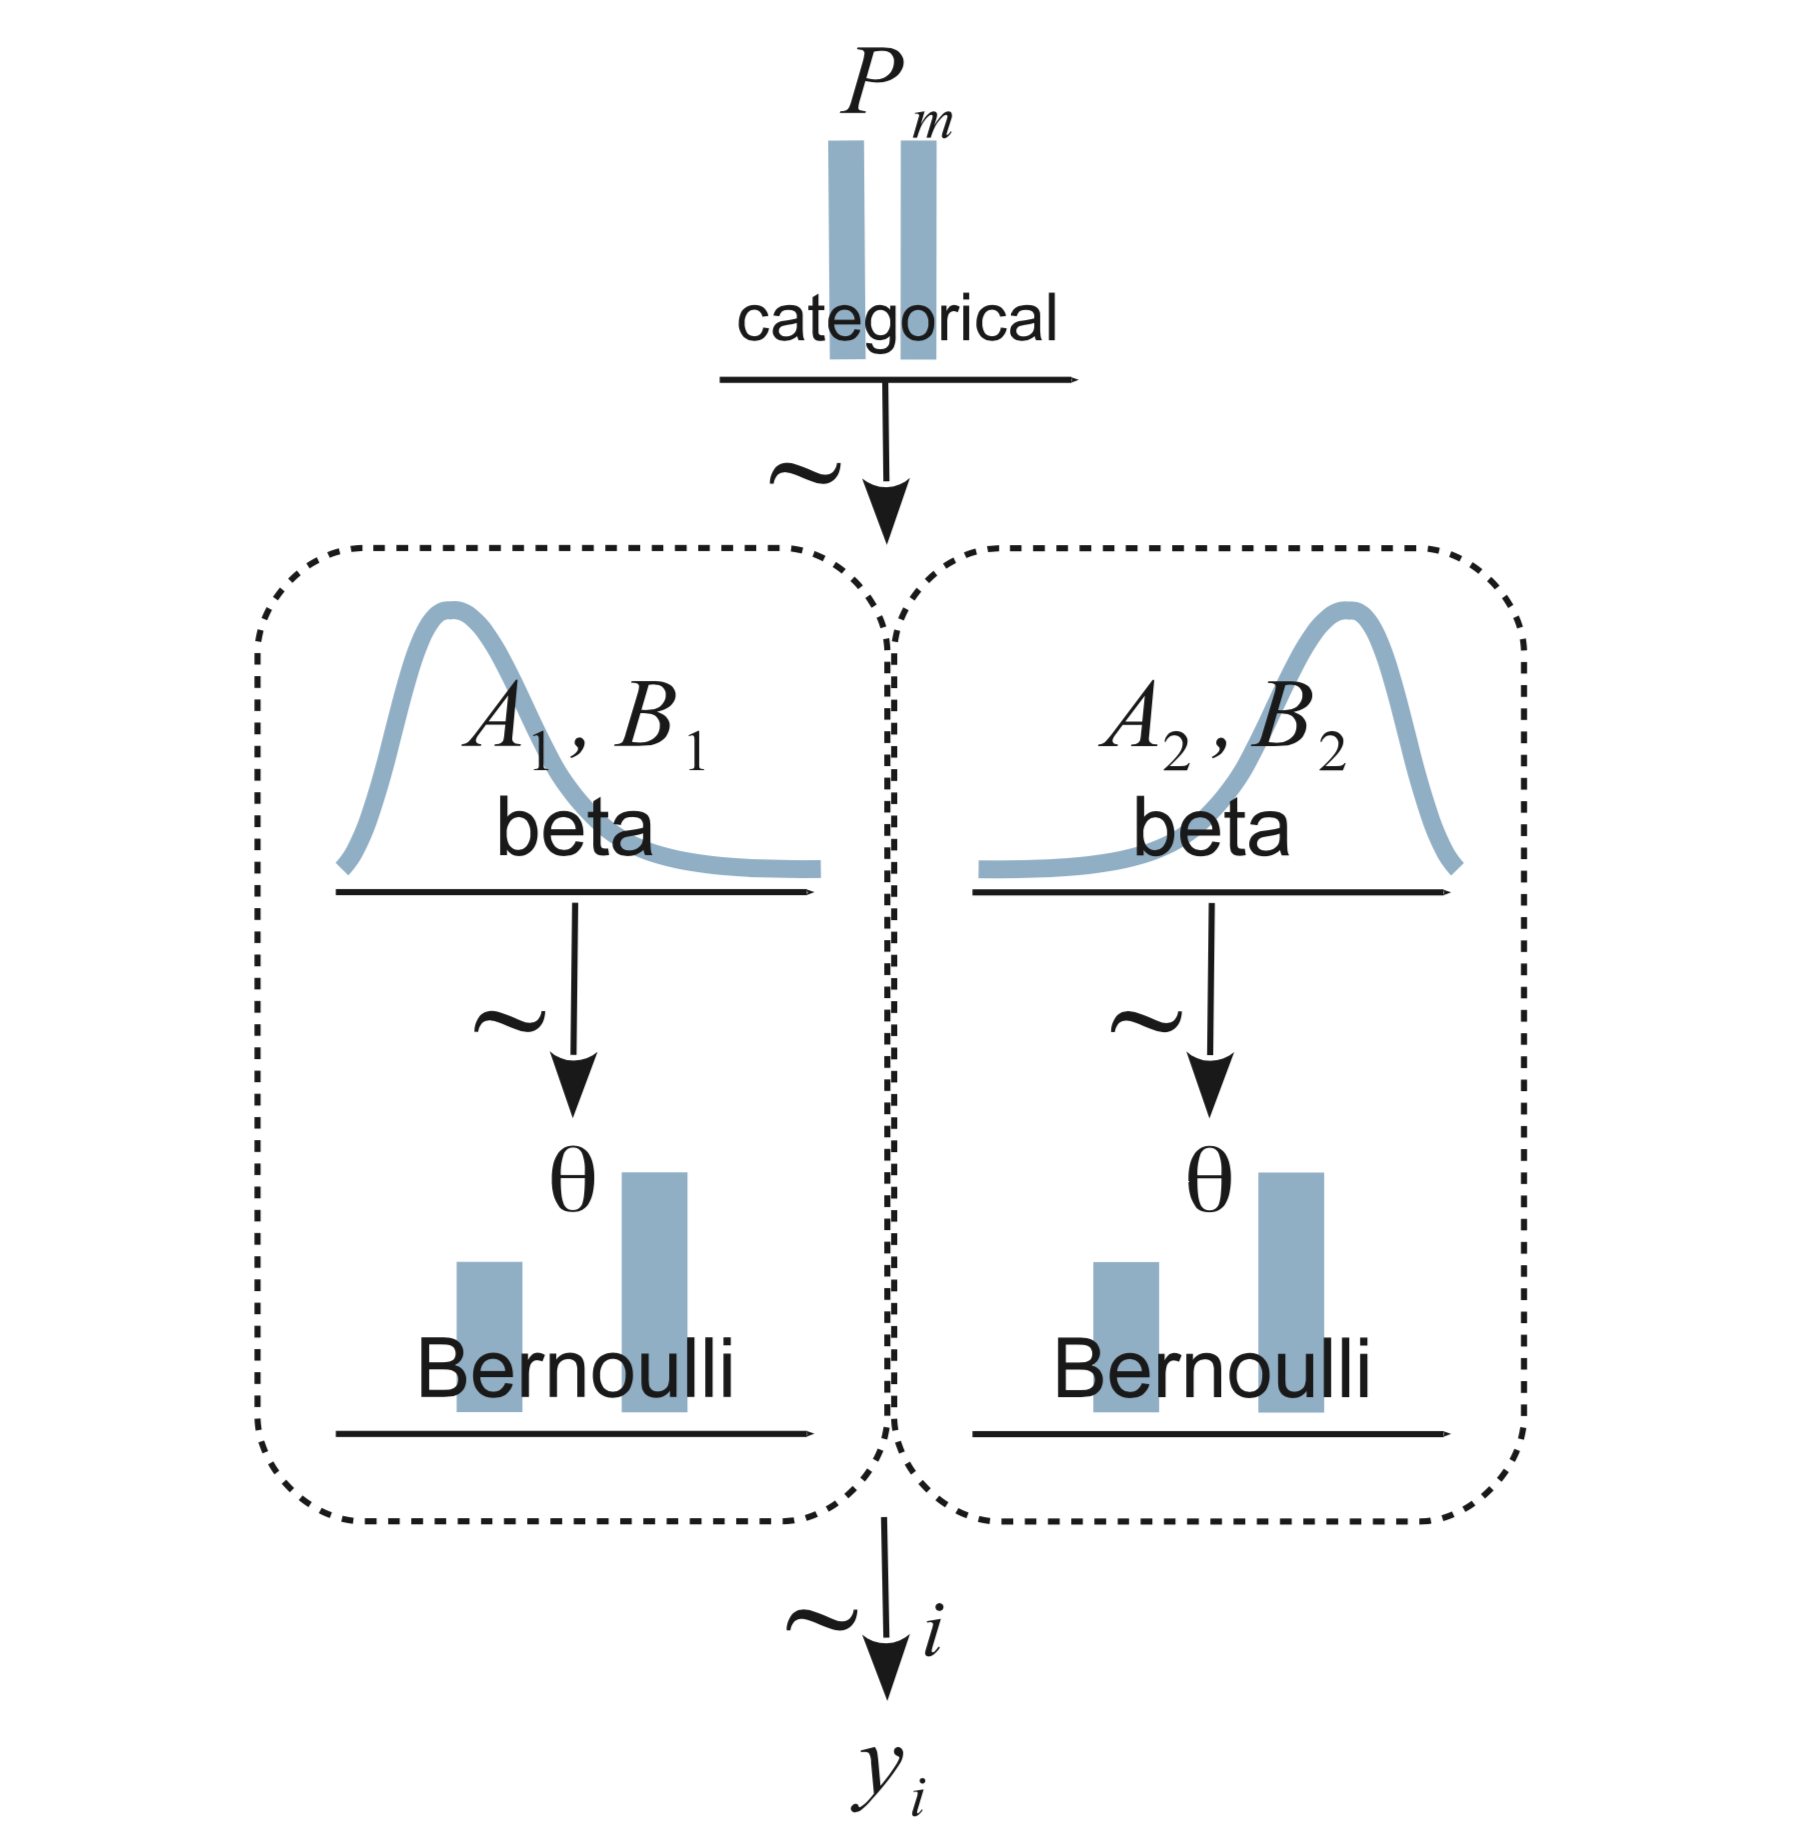
\includegraphics[width=0.8\textwidth]{coin_model_hierachy}
            \caption{Coin Model Hierachy}
            \label{fig:coin_model_hierachy}
        \end{figure}
\end{itemize}
\subsection{MCMC Method: Individual models}
\begin{itemize}
    \item Main formula to compute the probability of the data is:
    \[
        \frac{1}{p(D)} = \frac{1}{N} \sum_{n=\theta_{i} \tilde p(\theta|D)}^{N} \frac{h(\theta_{i})}{p(D|\theta_{i}) p(\theta_{i})} 
    .\]     
\item $h(\theta_{i}$ is a probability density function. There is a complex derivation to this formula, which we are skipping for now. Refer to page 275.
\end{itemize}
\subsection{MCMC Method: Hierachical model}
\begin{itemize}
    \item Similar to pymc3 models you have used. Use a index `m` to indicate for which model are the parameters being specified.
    \item The chain will be highly corelated with model index. 
    \item Chains will linger on one model for a long time. It will take a lot of iterations for the chains to explore both models equally.
    \item We can solve this using pseudo-priors.
\end{itemize}

\subsection{Why chains get stuck?}
\begin{itemize}
    \item At a step for which m=1, $\theta_{1}$ is used to descibe the data. However, $\theta_{2}$ is not bounded and is sampled randomly from prior. Vice-versa for m=2. 
    \item The prior might be very far away from the posterior. Because the other $\theta_{m = other}$ is a poor description of the data, the chain rarely jumps to it.
    \item \textbf{Solution}: For the parameter currently not being used, make it mimic the posterior. This way, it will always stay in the credible range of values.
\end{itemize}
\subsubsection{Values for pseudopriors}
\begin{itemize}
    \item Do initial run with pseudo prior set to true prior. Note characteristics of marginal distribution of the posterior. 
    \item Set pseudoprior values that mimic the current posterior. Run analysis and do step 1 again. Repeat this analysis if the pseudo-prior values are very different from the previous values you had.
\end{itemize}
\subsection{Model Averaging}
\begin{itemize}
    \item Instead of picking the best model that we got from the posterior analysis, we should instead do a weighted average of all the models.
    \item This is because our initial hierachical model took into account the posterior distributions from all models, rather than one single model.
    \item We can obtain this by using the following formula for the weighted averages:
    \[
        \sum_{m} p(\hat{y}|D, m) p(m | D)
    .\] 
    \[
        = \sum_{m} \int d \theta_{m}p_{m}(\hat{y}|\theta_{m}, m)p_{m}(\theta_{m}|D, m) p(m|D)
    .\] 
    This is called \textbf{model averaging}.
\end{itemize}
\subsection{Accounting for model complexity}
\begin{itemize}
    \item Complex models can find relationships between more variable BUT are more sensitive to noise.
    \item We need a way to measure model complexity, since the noisy data will always prefer more complex models(overfitting).
    \item Simple models can win if the data is in the same range the prior. This is because in simple models, the prior is restricted to a specific parameter space. In complex models, because the prior is spread over a very large space, the posterior distributions are not as strong as the simple model.
\end{itemize}
\subsection{Comparing nested models}
\begin{itemize}
    \item Suppose there is a model with many parameters that can describe the data very well.
    \item Now, we define some restrictions on the above parameters(lower bound 0, setting them equal to each other, etc.)
    \item Such a model can be "nested" in the original model.
    \item Here, the Bayesian model comparison will prefer the restricted model, because the full-model has a large prior diluted parameter space.
    \item \textbf{If prior probability of model is 0, then posterior probability is also 0.}
\end{itemize}
\subsection{Sensitive to prior distribution}
\begin{itemize}
    \item Bayesian model comparison is extremely sensitive to the prior distribution.
    \item Different priors and yield different Bayes factor's. 
    \item For uninformative priors, prefer \textbf{Haldane's prior}
    \item For Haldane's prior, the parameters are very close to 0. It is still a beta distribution. 
        \[
        a = b = 0.01
        .\] 
\end{itemize}
\end{document}
